\newcommand{\nomedoc}{User's Guide}
\newcommand{\versione}{1.0}
\newcommand{\versioneglossario}{3.0}
\newcommand{\versionenormeprogetto}{3.0}
\newcommand{\nomefile}{User's Guide-\versione.pdf}
\newcommand{\datacreazione}{24 Febbraio 2011}
\newcommand{\datamodifica}{27 Febbraio 2011}
\newcommand{\stato}{formale}
\newcommand{\uso}{esterno}
\newcommand{\redazione}{}
\newcommand{\verifica}{}
\newcommand{\approvazione}{}
\newcommand{\distribuzione}{
VT.G \\
& Prof. Vardanega Tullio\\
& Prof. Cardin Riccardo }

% FUNZIONI TIPOGRAFICHE
\newcommand{\co}{\texttt} % courier
\newcommand{\bo}{\textbf} % bold
\newcommand{\pr}{\par\medskip} % paragrafo spaziato
\newcommand{\sca}{\textsc} % small caps

\documentclass[a4paper,12pt]{report}
% 10pt,11pt,12pt
% titlepage, notitlepage -> per dare inizio o no ad una nuova pagina dopo titolo
% twoside -> per dire se fronte-retro
\usepackage[latin1]{inputenc}
% per caratteri accentati
\usepackage[italian]{babel}
% per regole sintattiche italiane
\usepackage[bookmarks=true, pdfborder={0 0 0 0}]{hyperref}
% per collegamenti ipertestuali
\usepackage{graphicx}
% per inserimento immagini

% \usepackage{enumerate}
% per personalizzare elenchi puntati

\usepackage[hmargin=2cm]{geometry} %margine 2 cm
%\geometry{options varie}

% comandi per gestire meglio header e footer
\usepackage{fancyhdr}  % header e footer
\usepackage{totpages}
\pagestyle{fancy}
\renewcommand{\headrulewidth}{0.4pt}
\renewcommand{\footrulewidth}{0.4pt}

\setlength{\headheight}{1.2cm} % NON TOCCARE
\setlength{\voffset}{-1.5cm} % NON TOCCARE
\setlength{\textheight}{666pt} % NON TOCCARE
\setlength{\footskip}{60pt}
\setlength{\parindent}{0pt} % INDENTAZIONE

\lhead{\nomedoc\  (ver. \versione)}
\chead{}
\rhead{
\includegraphics[height=1cm]{img/netmus.png}}
\lfoot{
\includegraphics[height=0.8cm]{img/logo.png}}
\cfoot{}
\rfoot{\thepage}

\usepackage{titlesec}
\titleformat{\chapter}{\normalfont\huge\bfseries}
{\thechapter}{20pt}{\Huge}

\usepackage{rotating}   % PER TABELLE E AMBIENTI RUOTATI
\usepackage{array}
\usepackage{color}
\usepackage{colortbl}  % VARIE PER GESTIRE I COLORI
\definecolor{Orange}{RGB}{255,127,0}   % ARANCIO ACCES0
\definecolor{orange}{RGB}{255,207,80}  % ARANCIO TENUE

\addtocontents{toc}{\protect\thispagestyle{fancy}}  % PER INDICI CON + PAGINE
\usepackage[font=it]{caption}    % PER RENDERE CORSIVE LE DIDASCALIE
\usepackage{eurosym}  % PER SIMBOLO EURO

% \usepackage{listings}   per codice sorgente

\author{VT.G - Valter Texas Group}

\begin{document}

\pagenumbering{Roman} % INIZIO NUMERAZIONE ARABA

\vspace*{1cm}
\begin{center}


\includegraphics[width=9cm]{img/logo.png}\\
\vspace{0.5cm}
\begin{LARGE} \sca{VT.G - Valter Texas Group} \end{LARGE}\\
\vspace{0.5cm}
\begin{Large}
\emph{valtertexasgroup@googlegroups.com} \end{Large}\\
\vspace*{1cm} 
\includegraphics[width=5cm]{img/netmus.png}\\
\vspace{0.5cm}
\begin{Large} \sca{\nomedoc} \end{Large}\\
\vspace{1cm}
\begin{Large} \emph{Ingegneria del Software A.A. 2010-2011} \end{Large}\\
\end{center}
\vspace{1cm}

% INFORMAZIONI DOCUMENTO
\begin{center}
\begin{tabular}{r|l}
\hline & \\
\bo{Name} & \nomefile \\
\bo{Current Version} & \versione \\
\bo{Creation} & \datacreazione \\
\bo{Last Modify} & \datamodifica \\
\bo{State} & \stato \\
\bo{Use} & \uso \\
\bo{Editing} & \redazione \\
\bo{Control} & \verifica \\
\bo{Approbation} & \approvazione \\
\bo{Distribution} & \distribuzione \\
& \\\hline
\end{tabular}
\end{center}
\newpage

\chapter*{Summary}
\thispagestyle{fancy}
This document is a simply and intuitive guide for beginners using NetMus
system.\\
It includes a glossary where you can find more-difficult terms that are used
here and an appendix whith the most common promblems that you can encounter,
possible reasons that caused the problem and possible solutions. 

\newpage
% REGISTRO MODIFICHE
\section*{Change History Log}

\begin{longtable}{|p{0.13\textwidth}|c|p{0.2\textwidth}|p{0.46\textwidth}|}
\hline
\rowcolor{orange} \bo{Data} & \bo{Version} & \bo{Author} & \bo{Description} \\
\endhead
\hline 
08/02/2011 & 0.1 & Lovato Daniele & Creation of the document.\\
\hline

\end{longtable}

% INDEX
\tableofcontents

\chapter{Introduction}
\thispagestyle{fancy} % serve perche' nelle pagine di inizio Chapter esca header e footer
\pagenumbering{arabic} % INIZIO NUMERAZIONE NORMALE
\rfoot{\thepage\ di \pageref{TotPages}}
This guide was created for beginners that want start using \co{NetMus}, and it
includes a description of the product and the instrutions for use it. There are
also two appendix in where you can find most common error messages and a
glossary.\\

All the terms in the glossary are underlined in the document in their first
occurence \underline{like this}.

\section{Description of the Product's User}
\co{NetMus} can be used by everyone: you need to know only the basics like using
a \underline{web browser} and navigating through internet. 


\section{How to Read this Guide}
This Guide presents the product \co{NetMus} and describes its functionality and
also the user's approach using the system. In particular it will show the 
actions that you can perform with the software and how to resolve, if it is
possible, problems that you can encounter using it.

\section{Helpful Documents}
Here we present the documents that we have used for writing this guide, and that
you can use to understand more clearly this words:
\begin{itemize}
  \item Analisi dei requisiti v3.0
  \item Norme di progetto v3.0
  \item Piano di progetto v3.0
  \item Specifica tecnica v2.0
  \item Definizione del prodotto v1.0
  \item Piano di qualifica v3.0
  \item Verbale 1 v1.0
  \item Capitolato C2 - NetMus del corso di Ingegneria del Software, A.A.
2010/11 (you can read it at the link 
\url{http://www.math.unipd.it/~tullio/IS-1/2010/Progetto/NetMus.pdf})
\end{itemize}

\section{How to report problems and not-working situations}
If you found any problems you can report it with the online service provided by
Google at this link:  \url{http://code.google.com/p/netmus/issues/list}.\\
You just have to click on top-left button \emph{New issue} and fill the
fields with a name for the problem and a short description of it.
If you want an help in descripting the problem, you can use the template
\emph{Defect report from user} that contains a track that help you writing all
the necessary informations. 

\chapter{General Description}
\thispagestyle{fancy}
Today, the biggest part of the population listen their music in Mp3 digital
format: it's for that reasons that was introduced \co{NetMus}, an useful
application that allows sharing our preferred music and listening it on online
streaming, and that was created with modern tecnologies like \underline{cloud
computing}.\\

\co{NetMus} allows to any user to have a virtual online library with all their
preferred songs, and to listen this songs everywhere and share them with
everyone.\\

This product is not only an online music library, but it has also a lot of
``\underline{social network}'' funcionalities that allows you to interact with every other user
registered to the system. So it's possible to view other users' music library
and listen their own songs, and also it's possible to make your own friend list
with all the other users registered to the system.\\

Using the product is very simple. Just after you get logged to \co{NetMus} you
only have to connect your PC with your Mp3 player and the system will start
working automatically. Otherwise you can also scan a local directory of your PC
that contains music in the mp3 format: all the songs will be fully extracted,
analyzed and inserted in your profile on your \co{NetMus} account, ready to be
listened.\\

Between \co{NetMus}' funcionalities we have streaming youtube player for audio
and video broadcasting, possibility to create your own playlists, and many other
utilities.\\

All the system is decorated with a graphical interface  too simple and intuitive
with the complete access to all the necessary funcionalities.\\


\chapter{Using Instructions}
\thispagestyle{fancy}

\section{Functional Description}
In this chapter we show a complete guide for \co{NetMus} use.\\
You will find a section were are listed all the required tools for a well
working approach with \co{NetMus}, then you will encounter a detailed overview
of \co{NetMus} with the description of all the actions you can perform with the
application.

\subsection{Recommended System Requirements for NetMus Use}
\co{NetMus} is a web application that is viewed and used with your web browser.
Although you reached it by internet navigation, you don't need only an internet
connection and a web browser to use it.\\

Now we show a list of the required tools that you need for use \co{NetMus}.

\begin{itemize}
  \item Internet Connection (higher than 56k)
  \item Web Browser (Google Chrome, Safari, Opera, Firefox*, IE**)
  \item A JVM (Java Virtual Machine) correctly installed on your PC
  \item Adobe Flash Player plugin for video broadcasting
  \item Javascript activated on your web browser
\end{itemize}

Without anyone of this tools you will not able to use
correctly all the system functionalities, or even you will unable to use
\co{NetMus} at all.\\
\\
\\

\emph{* If you use Firefox, you won't see the animation effects of the
system, because Firefox dosen't support the animations.}\\ 
\emph{** If you wanna use NetMus con Microsoft Internet Explorer, you have to
download the Google Chrome Frame plugin for IE, because this web browser doesn't
support the advanced funcionalities of NetMus.}\\

\section{Registering to NetMus}

Go at the link \url{http://netmusbeta.appspot.com} to start using \co{NetMus}.\\

\begin{figure}[htbp]
  \centering
  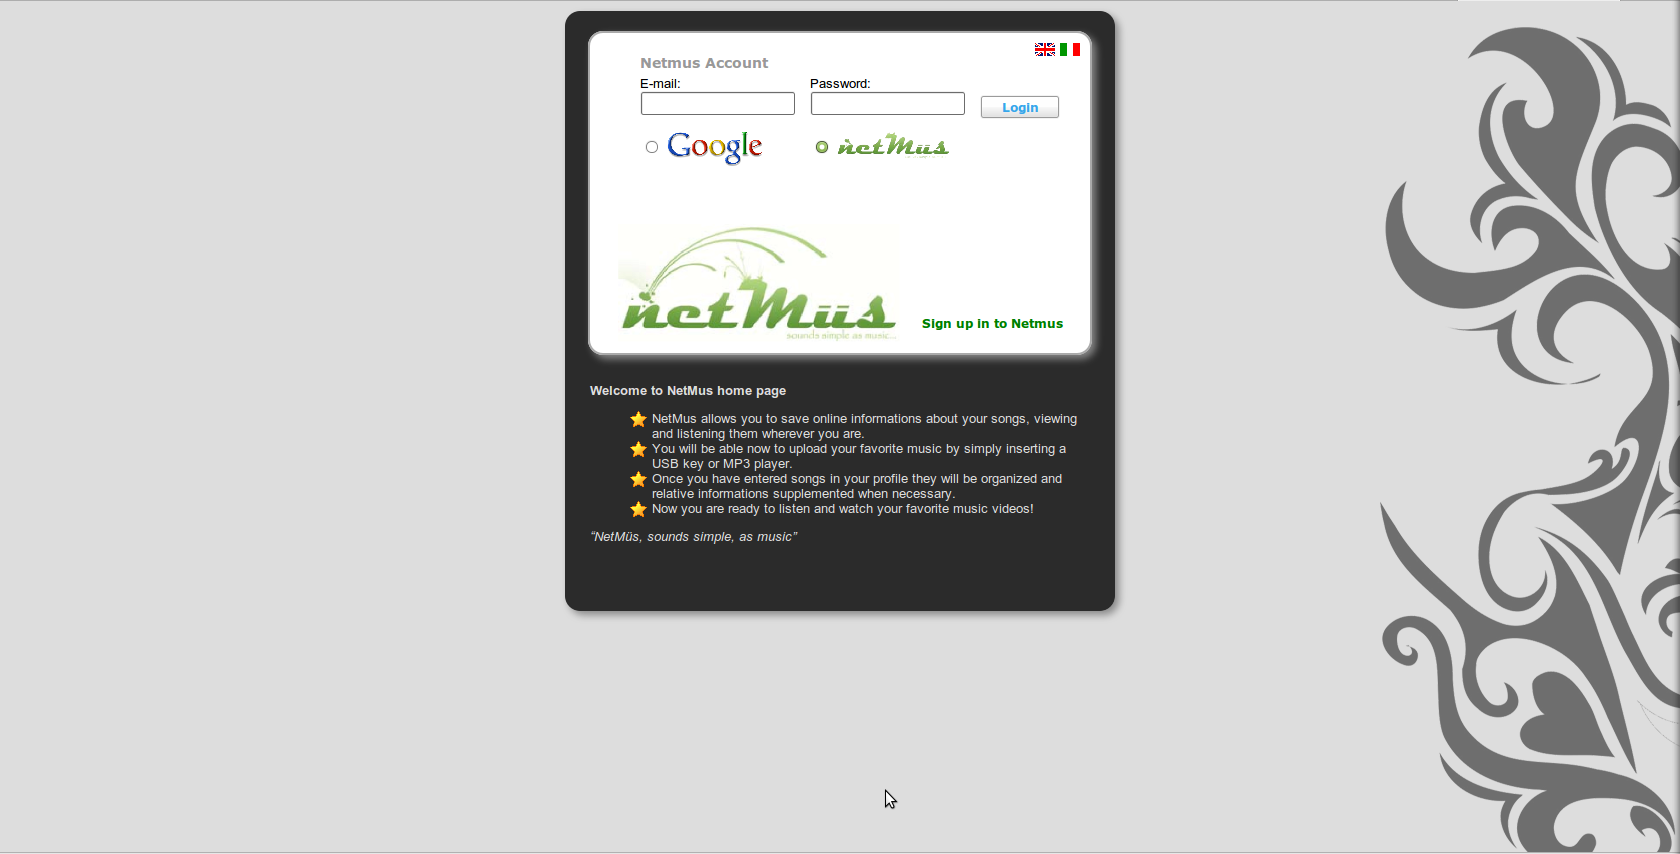
\includegraphics[width=15cm]{img/MU/login.png}
\caption{Netmus Login View}
\end{figure}


Here is the login page to enter \co{NetMus}. If you are already registered to
Google, you can enter in \co{NetMus} using your Google account.

You have to select the Google login and click on the button ``Log in
NetMus using your Google Account''. You will be redirected to the Google login
page, here you get logged in and then you will be redirected again to
\co{NetMus}, but this time you will be logged to the system.\\

\begin{figure}[htbp]
  \centering
  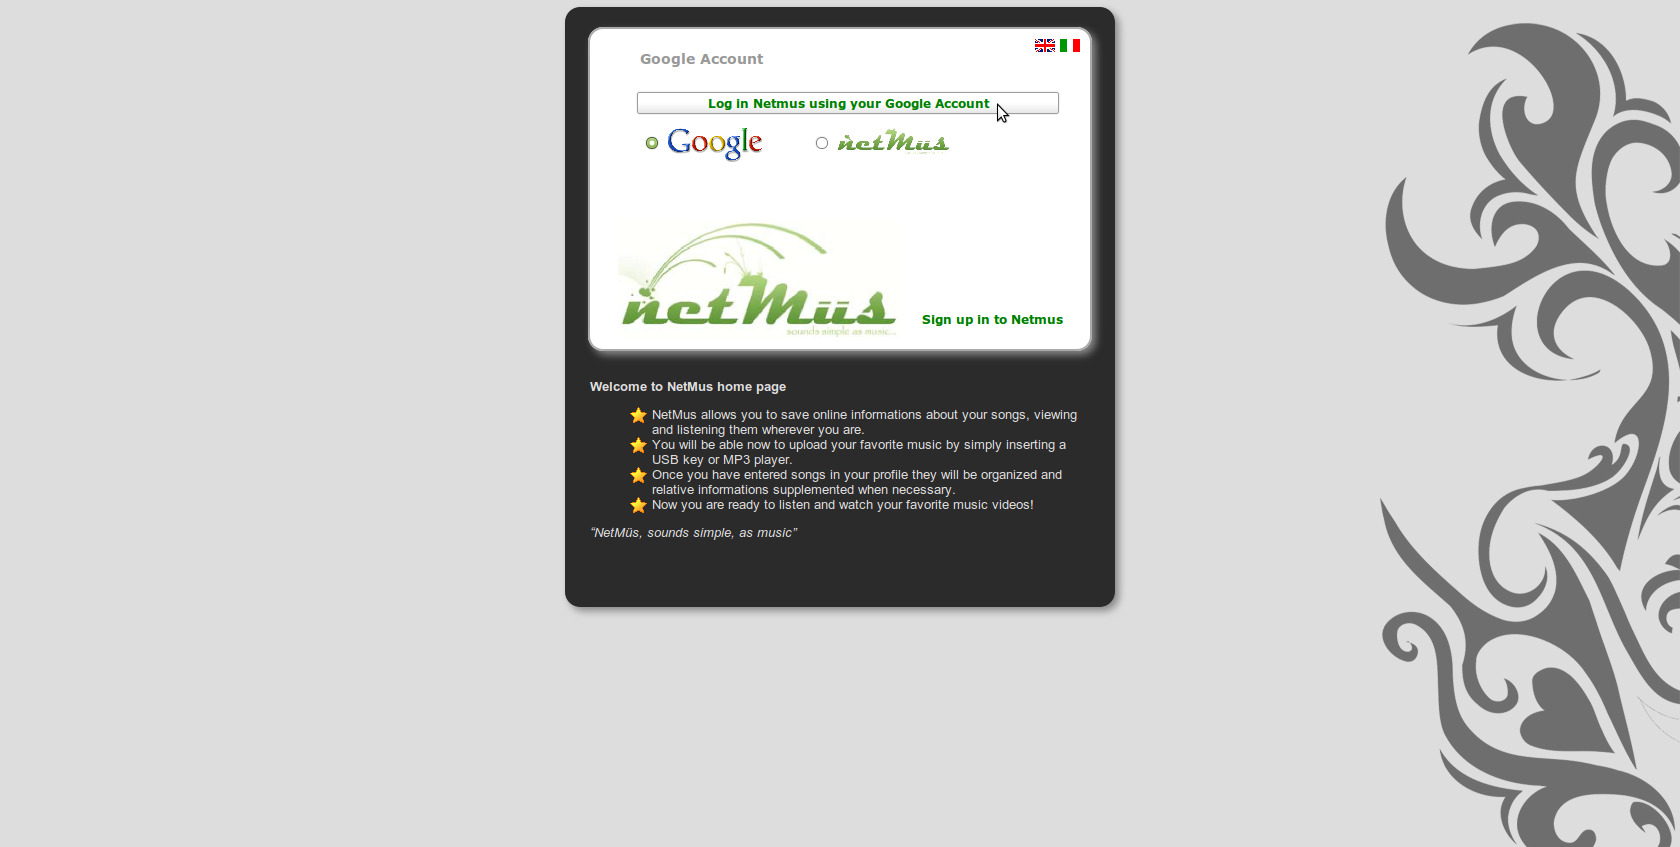
\includegraphics[width=15cm]{img/MU/loginGoogle.png}
\caption{Google Login View}
\end{figure}


If you aren't Google users and this si your firts access to \co{NetMus}, it
necessary that you create your own account registering to the system.
\co{NetMus} registration and use are completely free. \\

\begin{figure}[htbp]
  \centering
  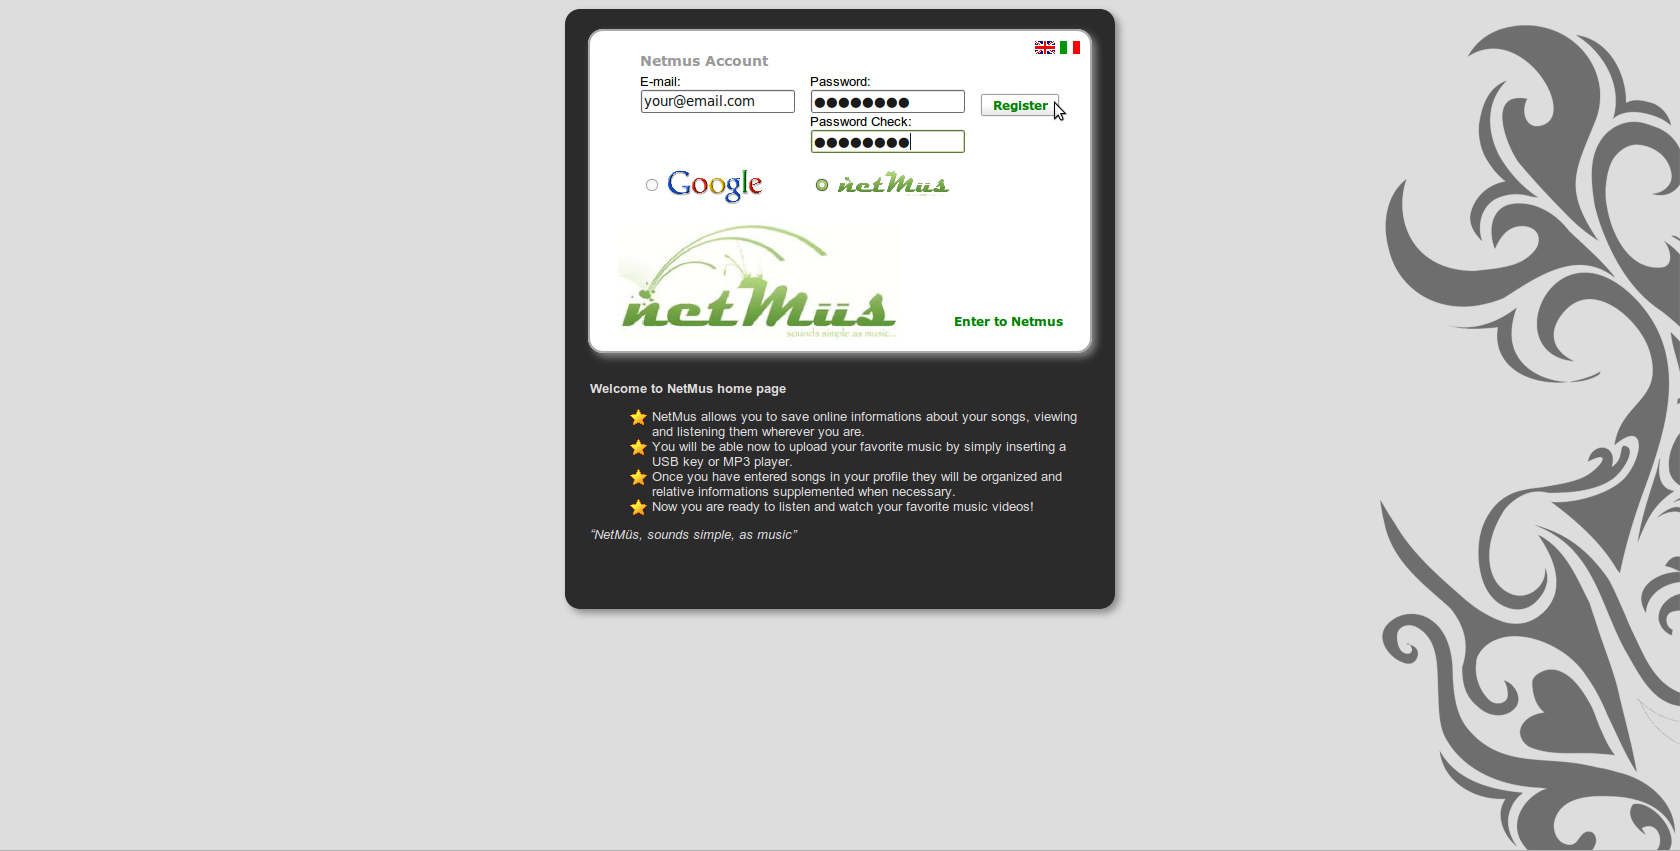
\includegraphics[width=15cm]{img/MU/registration.png}
\caption{Registration View}
\end{figure}


Registering yourself to the system you need to insert a correct email address
and a password with more than 5 characters. An email will be sent to your email
address for the confirmation of your account's activation.

\subsection{First Access to NetMus}

At your first access, the view that will be presented to you will be like that.

\begin{figure}[htbp]
  \centering
  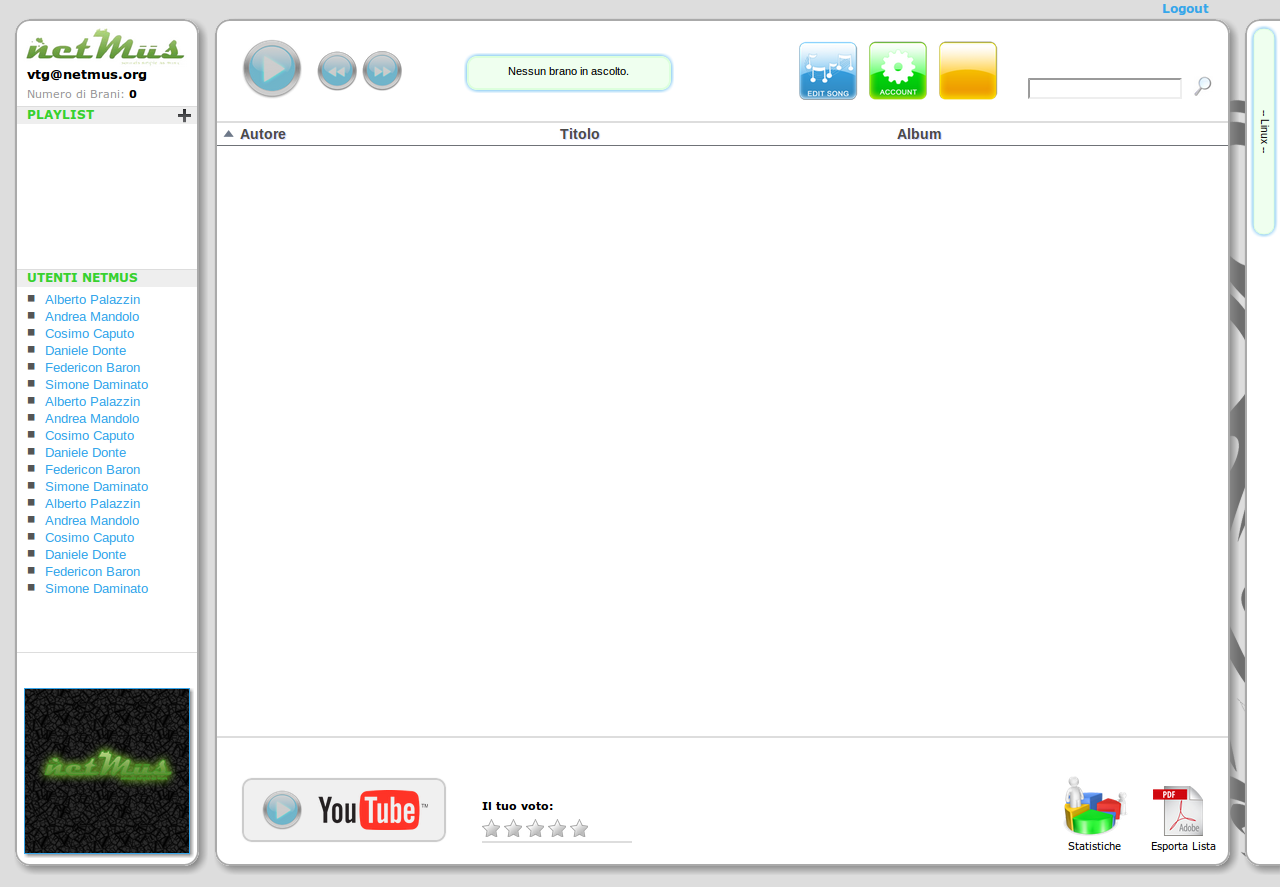
\includegraphics[width=15cm]{img/MU/profile_blank.png}
\caption{NetMus Homepage at first access}
\end{figure}

Beginning from the left, we find a menu that presents the \co{NetMus} logo and
your \underline{nickname}, that for now is your email address. It also presents
the number of songs contained in your songs' list, that are zero at your first
access. This is playlist menu, infact here we can find all the playlist you have
created, and it also leads creating new ones by clicking on the red ``+''
symbol.\\
\\
The central section is the most important part of the apllication, infact this
is our music library with youtube player and other buttons for other
funcionalities.\\
\\
At the right side of the page there is a bar called ``DEVICE SCANNER BAR" that
allows the scanning process of the \underline{mass storage devices}. If you
hover this bar with your mouse pointer, the bar will expand revealing many details: a label were is
written  the scanning process status and a button for the manual scanning
process of an arbitrary directory selected.\\

\begin{figure}[htbp]
  \centering
  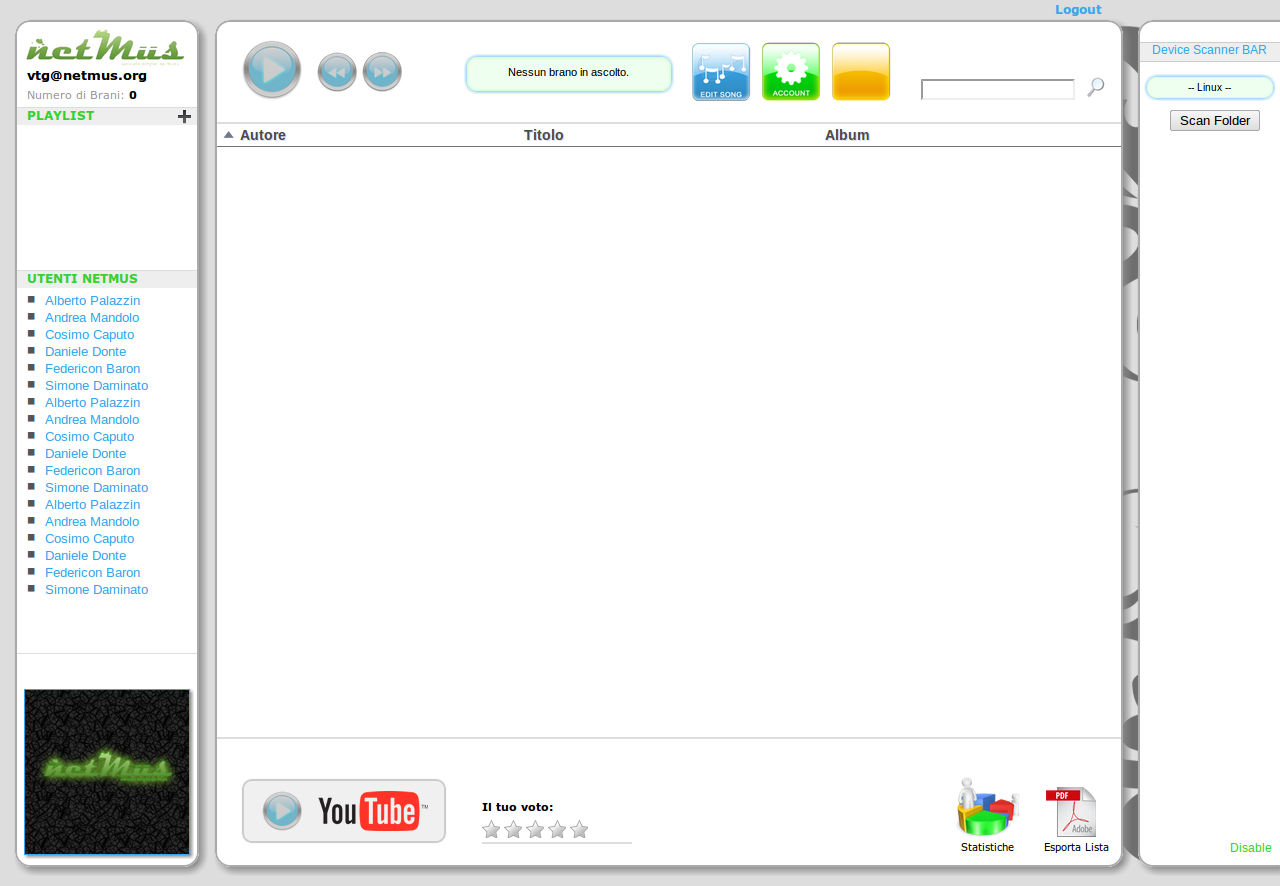
\includegraphics[width=15cm]{img/MU/applet_bar_open.png}
\caption{NetMus homepage with expanded DEVICE SCANNER BAR}
\end{figure}

\subsection{Start Using NetMus}

First of all if you want to take advantage of the main \co{NetMus}' peculiarity,
the online music library, it necessary that you put an USB device in your PC.\\
Otherwise it is possible to scan a selected directory of your own PC, clicking
on the ``Scan Folder'' button for manual selection of the directory.\\ 

\begin{figure}[htbp]
  \centering
  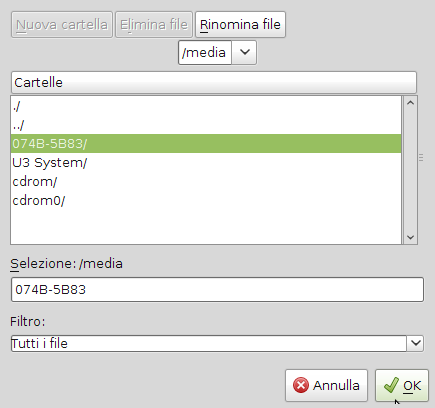
\includegraphics[width=15cm]{img/MU/scan_manual.png}
\caption{Manual Scanning View}
\end{figure}

When the analysis starts you can follow the process in the DEVICE SCANNER BAR
inside its label that shows the numbers of the files that are analyzed until
appeared the message ``Sending Done'' that indicates that all the files have
been sent to the music library.\\

\begin{figure}[htbp]
  \centering
  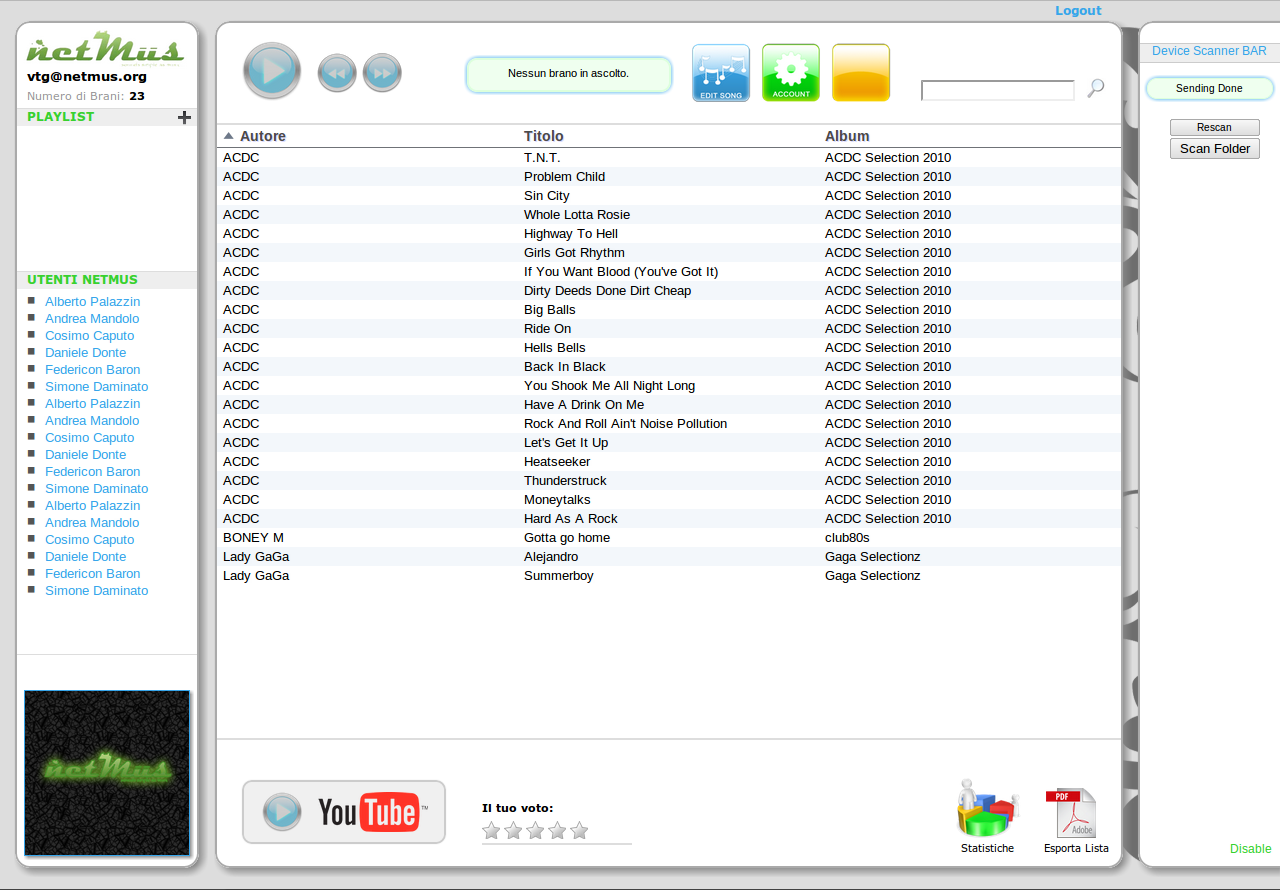
\includegraphics[width=15cm]{img/MU/song_loaded.png}
\caption{View with some songs on the Music Library}
\end{figure}

Once the files have been sent they should appear inside your music library.\\
Now it's possible for you to start using \co{NetMus} funcionalities.\\
All the actions that you can perform to take advantage of \co{NetMus} are listed
in subparagraphs some lines below for searching and viewing comfort.


\section{Permitted Actions}
In the section below we present all the actions that you are allowed to perform
to take advantage of \co{NetMus} funcionalities.

\subsection{Display Modality}

The library is the central part of \co{NetMus}. Here you can find an ordinate
list of your songs saved by the scanning process of your devices. It's possible
to have two different views of the same library.\\
\\
The first is the list modality, that is the default modality. In this
way songs are listed with the informations about the title, the artist and the
album. You can also order your songs by clicking on the superior bar the voice
``artist'', ``title'', ``album''.\\

---------list view mode picture------------
\\

The second is the ``cover mode'' modality in wich your songs are listed with the
cover of their own album. This is a nicer way to view the songs, and it is also
a better way to recognized the same album's songs.\\

-------cover mode picture---------
\\

 \subsection*{Listening a song in streaming}

The first funcionality that we want to describe is the most interesting of the
product, the streaming funcionality.\\
If you want to listen one of your songs, you just have to select it from the
library, then click on tha play button of the top player, or the
bottom YouTube player.\\

The function of the two players is the same, but they have some differences.
Infact the first player at the top of the page allows to play a song, but also
allows to shift at the next song or the previous, meanwhile the bottom player
transforms itselfs in a YouTube streaming video player, where your selected song
is reproduced. Furthermore that player shows YouTube link to the video, and if
you click on it you will be redirected to the YouTube page of the song video.\\


\begin{figure}[htbp]
  \centering
  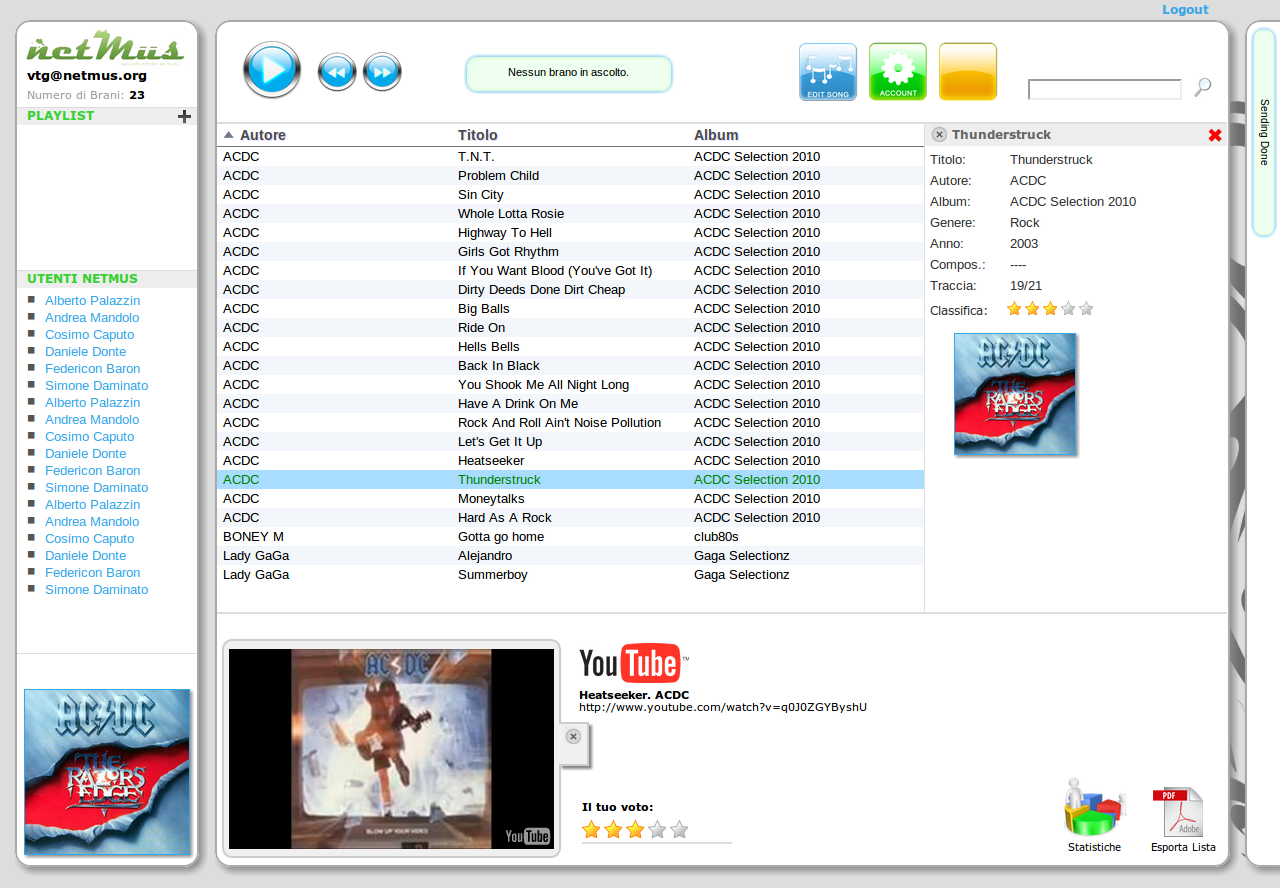
\includegraphics[width=15cm]{img/MU/player_youtube.png}
\caption{A video being reproduced with the YouTube player}
\end{figure} 

\subsection*{Create a Playlist}

Creating a \underline{playlist} is a very simple operation that allows you have
an ordinate sequence of your favorite songs.\\
If you want to create a playlist you just have to click on the ``+'' button on
the left menu near the voice ``PLAYLIST''. Just below it will appear a field in
wich you can enter the title of the playlist. Once you insert the title you push
enter button and the playlist will be created.\\

\begin{figure}[htbp]
  \centering
  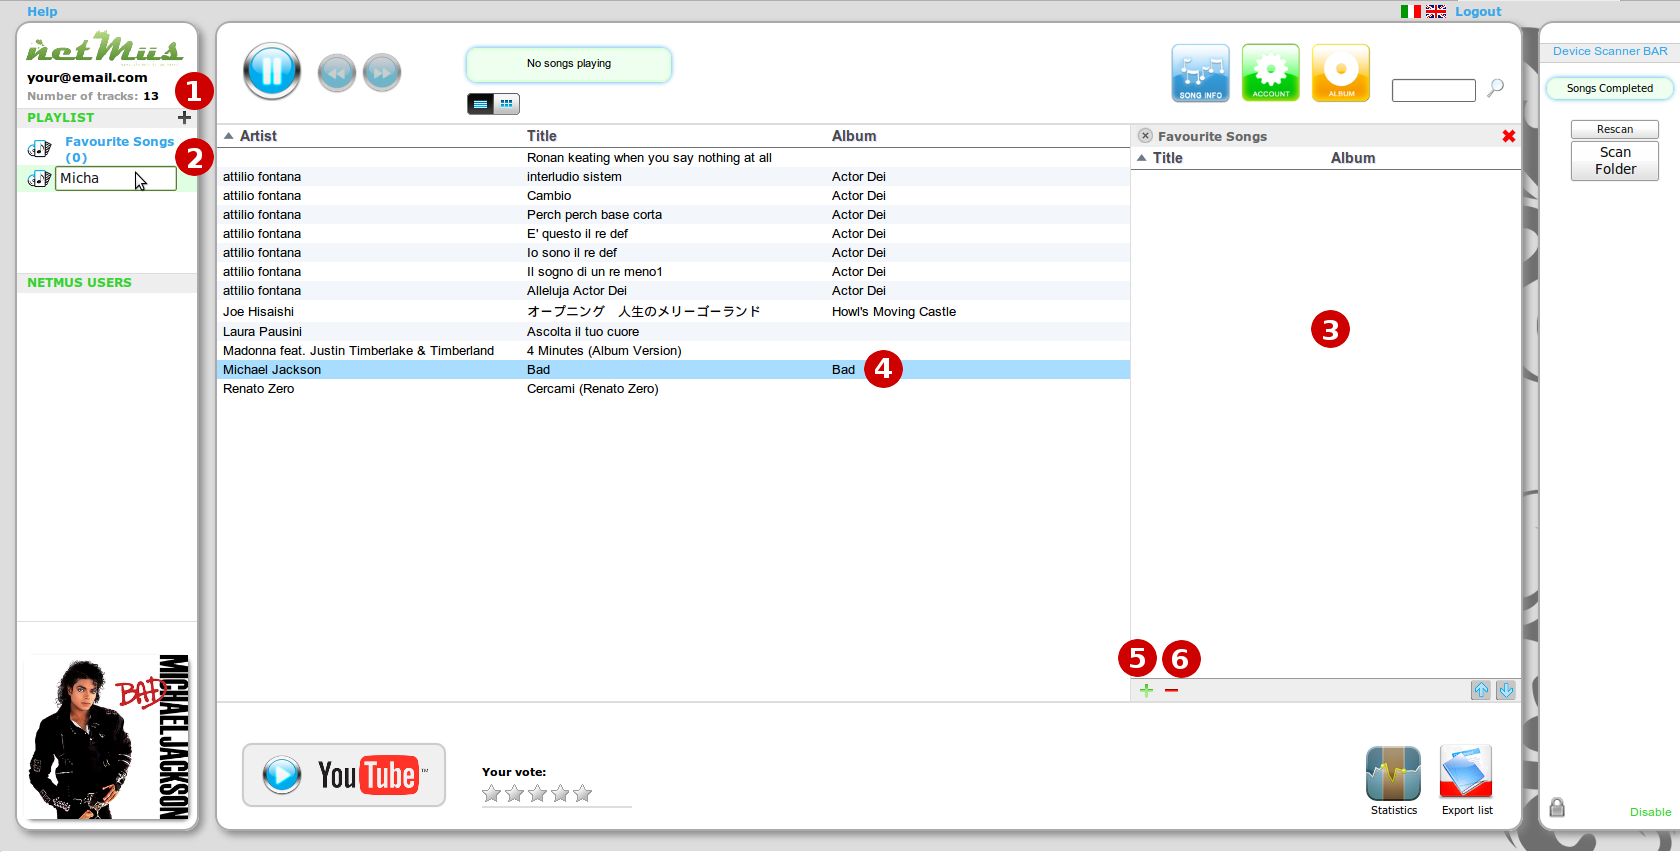
\includegraphics[width=15cm]{img/MU/new_playlist.png}
\caption{NetMus homepage with playlist menu}
\end{figure}

Now you just need to insert the songs that you want in your playlist. To do this
action you just have to click on the playlist name, it will appear a new window
empty for the moment, in where you will find all playlist's songs. To insert a
new song in the playlist you have to click on the ``+'' green button.\\
If you want to remove a song from the playlist you have to select from the
windows of the playlist the song you want to remove, and then click on the ``-''
red button.\\

\begin{figure}[htbp]
  \centering
  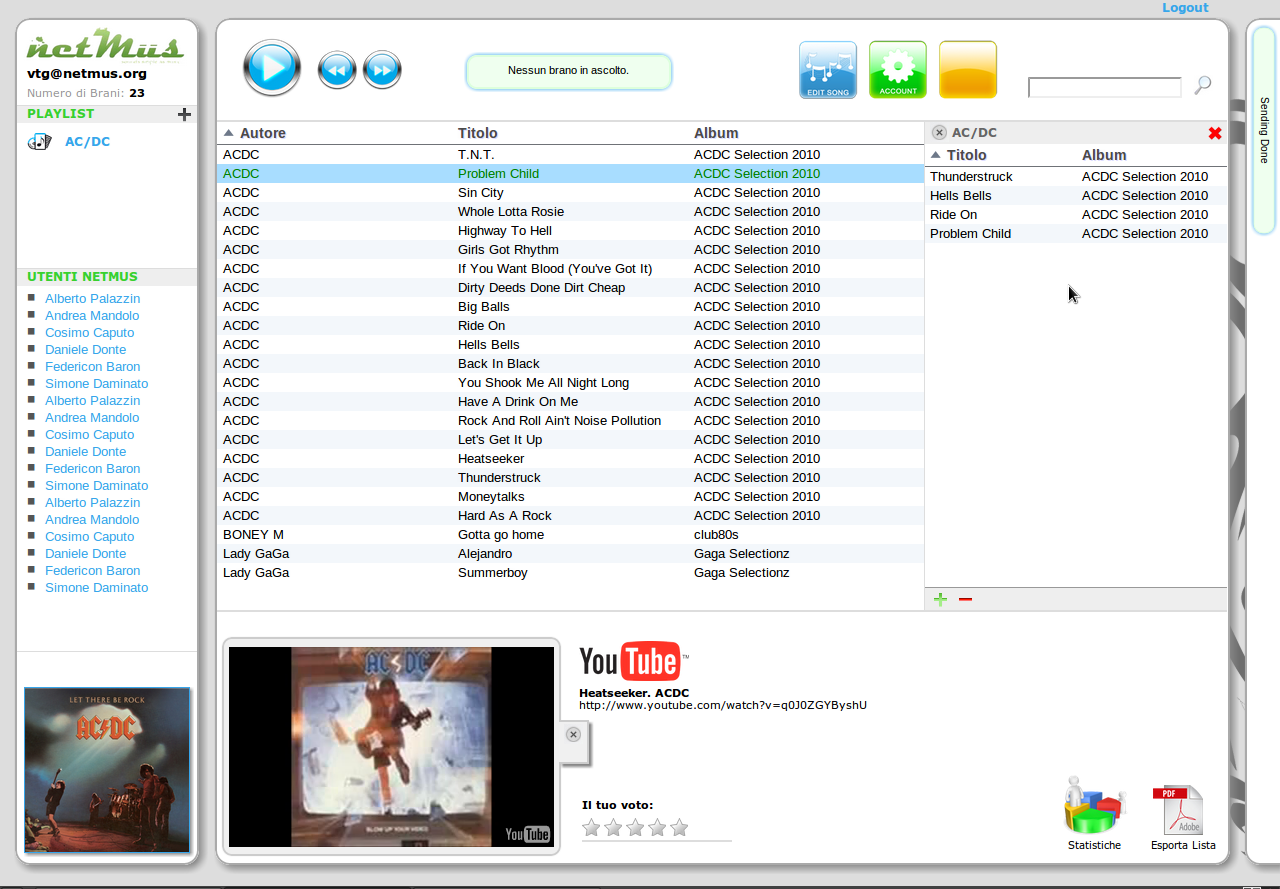
\includegraphics[width=15cm]{img/MU/playlist_song.png}
\caption{Playlist details}
\end{figure}

Finally if you want to delete a playlist you just have to click on the red ``X''
that is at the top-right side of the playlist details window.

\subsection*{Songs Details}

If you want to view all the informations complete about a song you just have to
do a double click on the same song. It will appear a small window with a list of
all the informations of the song.\\
\begin{figure}[htbp]
  \centering
  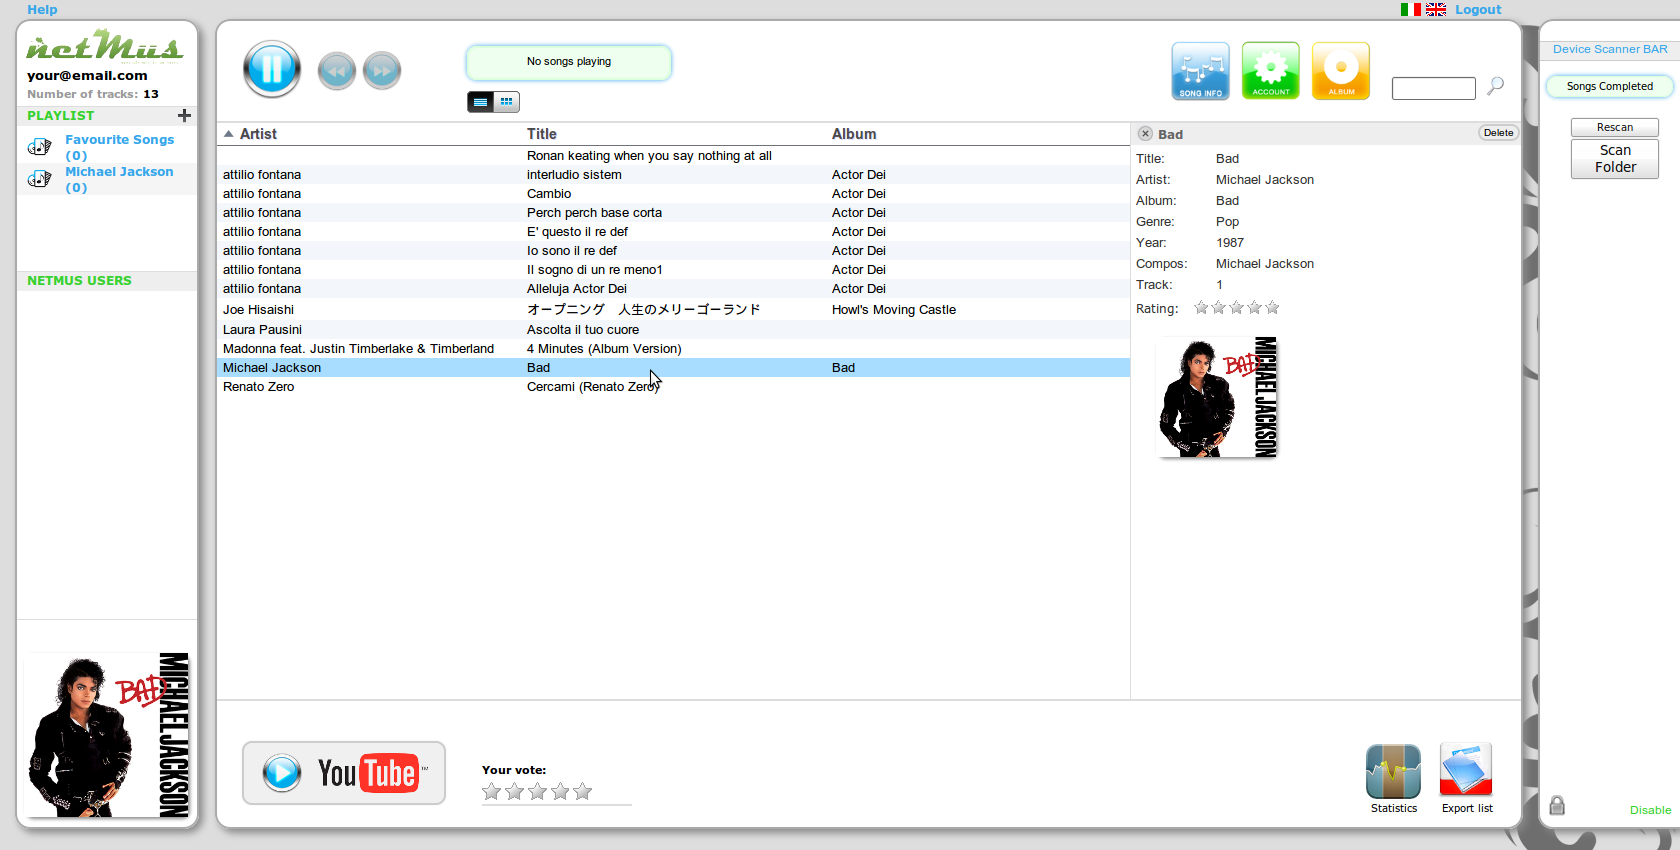
\includegraphics[width=15cm]{img/MU/info_song.png}
\caption{Song details}
\end{figure}

In the details you can see the song's title, author, album, genre, year,
composer, track number, evaluation and cover.\\
The evaluation is a funciontality that will be explained better in the next
paragraphs.\\
The covers are searched and saved when the songs are sent to the library.

\subsection*{Delete a song from your library}

To delete a song from your own library you just have to do a double click on the
song you want to delete. Then on the details window that appeared you have to
click on the red ``X'', and the song will be deleted from your library.

\subsection*{Searching a song on your library}

When you want to search a song in your library, you can use the right \underline{form}. This
form is placed on the top-right side of the page, and it allows to search a song
on your library only wrinting the title, album or artist's song. The searching
process is in real time, that means that all the results are shown in the center
library while you are typing.


\subsection*{Modify song's informations}

\subsection*{Modify your profile's informations (change password too)}

In the \co{NetMus} system it is possible add new informations about your
profile.\\
You can perform this operation by clicking on the green button ``Account''. It
will appear a pop-up with a list of informations that you can complete. These
informations had to be inserted in to their right form.

\begin{figure}[htbp]
  \centering
  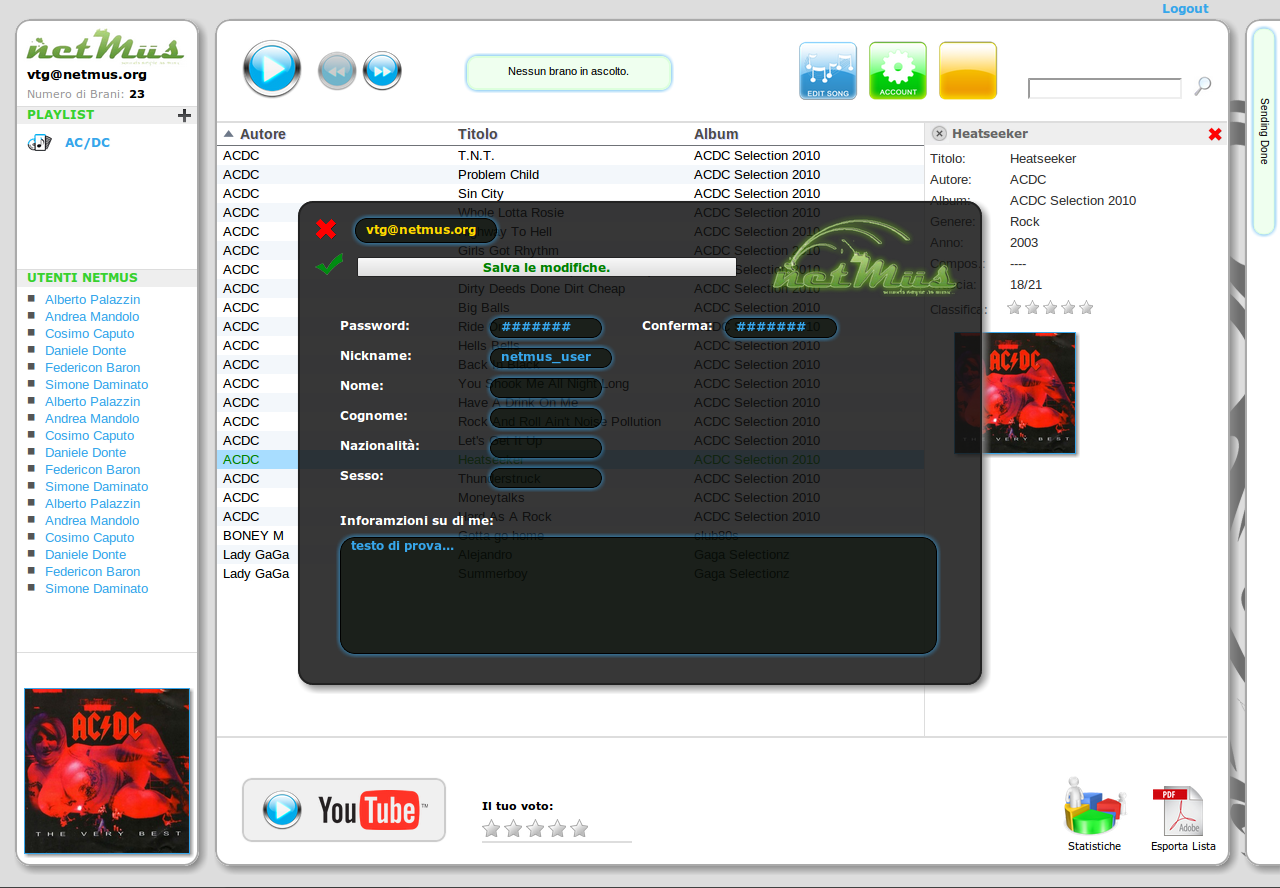
\includegraphics[width=15cm]{img/MU/profile_view.png}
\caption{View with the informations of the profile account}
\end{figure}

You can add to your profile a complete nickname, name, surname, nationality, sex
and a small description about yourself. From this view it's possible also change
your password.\\
When you have finished inserting all the informations you can click ``Save
changes'', or click on the red ``X'' to abort the operation.

\subsection*{Set rating for a song}

\co{NetMus} give you the possibility to set a rating to a song from zero to five
stars.\\
Your rating will be added to all the ratings given by all the other users who
have the same song on their library and the average of all the votes will appear
in the details of the song.\\
To set a rating you have just to select the song from the library, then click on
the star number that you want at the bottom side of the page. The rating will be
automatically registered in the informations of this song.

\subsection*{Creating a PDF of your music library}

This original funcion allows you to export your library to a PDF document that
you can later print.\\
You just have to click on the bottom-right side on the button ``Esporta Lista''
to create your document. When you have clicked, the system will automatically
generate a PDF document and it will appear a window where you have to select the
directory where the document will be saved.

\subsection*{View system and your account's statistics}


\newpage
\section{Errors and their Possible Reasons}

\subsection*{The USB device can't be scanned}
\begin{itemize}
  \item maybe the DEVICE SCANNER BAR isn't enable. Check on the DEVICE SCANNER
  BAR menu the label on the bottom-right side: the scanning process is disabled
  if the button displays the red word ``Enable''.
\end{itemize}

\subsection*{Some songs that were in the device haven't been stored in the
library}
\begin{itemize}
  \item maybe these songs had been analyzed some time before. To be sure of
  this, you can check the log that \co{NetMus} create inside your device with
  le list of the scanned songs.
  \item your mp3 songs hasn't all the most important tags complete. If an mp3
  file hasn't the tag artist, album and title complete with information, the
  song will not be stored on your library because it's impossible to identify
  what song is that.
  \item your songs has tags with an ecnoding type different from ISO-8859-1. A
  song with artist, album and title tags with a different encoding type will not
  be stored because the system doesen't recognize them. Songs with for example
  japanese tags will be ignored.
\end{itemize}

\subsection*{The song reproduced by the YouTube player is not the correct one}
\begin{itemize}
  \item the YouTube research funcionality not always produces correct results.
  It's possible listen the next song found by YouTube by clicking on the button
  ``Wrong Song''. With that funcionality there are more possibilities to find
  the correct song you want listen.
  \item the informations tag of this song are uncorrect, so the searching
  process couldn't find the correct song you want. Change the informations of
  this song to have a correct search answer from the player.
\end{itemize}

\subsection*{Forgotten password}

\appendix % inizio appendice
\chapter{Most Common Error Messages}
\thispagestyle{fancy}

\chapter{Glossary}
\thispagestyle{fancy}

\subsection*{Web Browser:} program that allows any user to navigate through the
internet. Internet Explorer, NetScape and Firefox are web browsers. 
\subsection*{Cloud computing:} a group of computer tecnologies that allows to
take advantage of many resources allocate in remote. 
\subsection*{Directory:}
folder of your PC. 
\subsection*{Mass storage devices:} external hard disk, USB pens, Mp3 players
exc. 
\subsection*{Form:} part of the graphical inteface, where you can insert some
text. 
\subsection*{Nickname:} user's name.
\subsection*{Playlist:} a song list that you can create to listen all the songs
that you like more and in the order that you prefer. 
\subsection*{Social network:} 
\subsection*{Streaming:} is a multimedia service that allows to see video and
listen audio files from a remote source thant sent all these informations to
many destinations through telecommunications network.

\end{document}